\section{图形的变换}

\item {
    $\bigstar\bigstar\bigstar$
    如图, 已知线段AB, 求作等腰直角三角形, 使其斜边等于线段AB, 保留作图痕迹并证明. \\
    \par\bigskip
    \begin{tikzpicture}
        % 带端点标注的线段
        \draw[|-|] (1, 0) -- (4, 0) 
            node[left] at (1, 0) {A}
            node[right] at (4, 0) {B};
    \end{tikzpicture}
    \ifshowSolution
        \fangsong\zihao{6}
        \\
        思路: 先满足等腰, 再满足直角. 

        正解:\\
        \begin{tikzpicture}
            % 带端点标注的线段
            \coordinate (A) at (0, 0);
            \coordinate (B) at (4, 0);
            \coordinate (O) at (2, 0);
            \coordinate (P) at (2, -4);
            
            \draw[|-|] (A) -- (B) 
                node[left] at (0, 0) {A}
                node[right] at (4, 0) {B};

            \draw (A) +(283:4. 47cm) arc (283:310:4. 47cm);
            \draw (B) +(231:4. 47cm) arc (231:258:4. 47cm);

            \draw[-] (2, 1) -- (2, -5);

            \draw (O) +(258:2cm) arc (258:278:2cm);

            \coordinate (C) at (2, -2);
            \draw[-] (C) -- (A)
                node[below left] at (C) {C};
            \draw[-] (C) -- (B);

            \fill (O) circle node[above left] {$O$};
            \fill (P) circle node[below left] {$P$};
        \end{tikzpicture} \\
        证明: \\
        (1) 先证明 $\triangle ABC$ 是等腰三角形. \\
         $\because OP$ 是 AB 的垂直平分线, 点 C 在 AB 上, \\
        $\therefore AC = BC$. \\
        (2) 再证明 $\triangle ABC$ 是直角三角形.\\
        $\because OA = OC = OB$, \\
        $\therefore \angle A = \angle ACO, \angle B = \angle BOC,$ \\
        $\therefore \angle ACB = \angle A + \angle B.$ \\
        $\because$ 三角形内角为 $180^\circ, $ \\
        $\therefore \angle ACB = 90^\circ.$ \\
        所以, $\triangle ABC$ 是等腰直角三角形.

    \else
        \\ \\ \\ \\ \\ \\ \\ \\
    \fi
}

\item {
    $\bigstar\bigstar$
    尺规作图. 已知$\triangle ABC$,作它的三个角的角平分线. 你有何发现?\\
    \begin{tikzpicture}[scale=1. 2]
    % 绘制角AOB
    \coordinate (A) at (2, 3);
    \coordinate (C) at (4, 0);
    \coordinate (B) at (0, 0);
    \draw (A) -- (B);
    \draw (C) -- (B);
    \draw (C) -- (A);
    % 标注点
    \fill (A) circle  node[above left] {$A$};
    \fill (B) circle  node[below left] {$B$};
    \fill (C) circle  node[below right] {$C$};
    \end{tikzpicture}
    \ifshowSolution
        \fangsong\zihao{6}
        \\
        % 思路: 
    \else
        \\ \\ \\ \\
    \fi
}

\item {
    $\bigstar$
    如图, $\angle AOB=45\degree$, 点$M, N$分别在射线$OA,OB$上,$MN=5, S_{\triangle OMN} = 15$, 点$P$是直线$MN$上的一个动点,点$P$关于$OA$的对称点为$P_1$,点$P$关于$OB$的对称点为$P_2$. 连接$OP_1, OP_2, P_1P_2$, 当点$P$在直线$MN$上运动时,则 $\triangle OP_1P_2$的面积的最小值是多少?此时点$P$ 在哪里? \\
    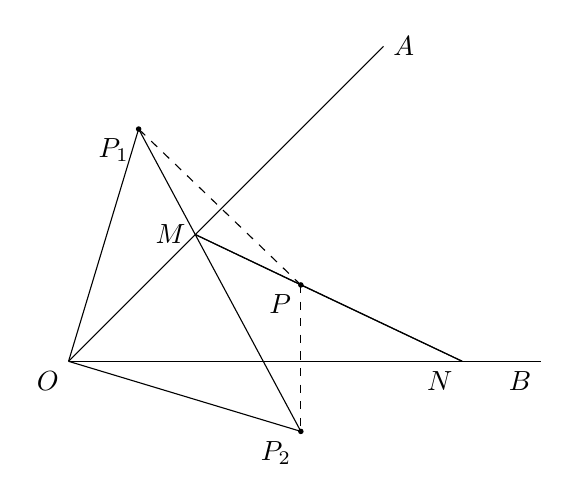
\begin{tikzpicture}[scale=1]
        % 绘制角AOB
        \coordinate (O) at (0, 0);
        \coordinate (A) at (4, 4);
        \coordinate (B) at (6, 0);
        \draw (O) -- (A);
        \draw (O) -- (B);
        
        % 标注点P
        \coordinate (P) at (2.95, 0.97);
        \coordinate (P_1) at (0.89, 2.95);
        \coordinate (P_2) at (2.95, -0.89);
        \draw [dashed] (P) -- (P_1);
        \draw [dashed] (P) -- (P_2);
        \draw (P_1) -- (P_2);
        \draw (O) -- (P_1);
        \draw (O) -- (P_2);
    
        \coordinate (M) at (1.61, 1.61);
        \coordinate (N) at (5, 0);
        \draw (M) -- (P);
        \draw (N) -- (P);
        \draw (N) -- (M);
    
        % 标注所有点
        node[left] at (0, 0) {A}
        \fill (O) circle  node[below left] {$O$};
        \fill (A) circle (0pt) node[right] {$A$};
        \fill (B) circle (0pt) node[below left] {$B$};
        \fill (P) circle (1pt) node[below left] {$P$};
        \fill (P_1) circle (1pt) node[below left] {$P_1$};
        \fill (P_2) circle (1pt) node[below left] {$P_2$};
        \fill (M) circle (0pt) node[left] {$M$};
        \fill (N) circle (0pt) node[below left] {$N$};
        \end{tikzpicture}
    \ifshowSolution
        \fangsong\zihao{6}
        \\
        % 思路: 18
    \else
        \\ \\ \\ \\ \\ \\
    \fi
}

\item {
    $\bigstar$
    如图,把一张长方形纸片$ABCD$沿$EF$折叠后$ED$与$BC$的交点为$G$,$D,C$分别在$M,N$的位置上,若$\angle EFG=55\degree$,则$\angle AEM$是多少度?\\
    \par\bigskip
    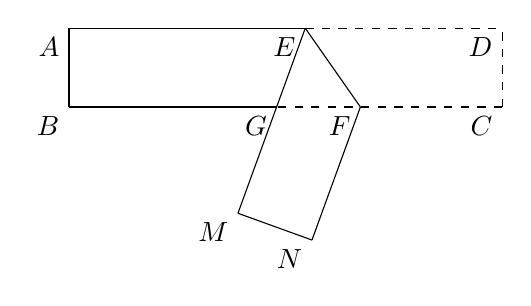
\begin{tikzpicture}[scale=0.5]
    \coordinate (A) at (-5, 1);
    \coordinate (B) at (-5, -1);
    \coordinate (C) at (6, -1);
    \coordinate (D) at (6, 1);
    \coordinate (E) at (1, 1);
    \coordinate (F) at (2.4, -1);
    \coordinate (G) at (0.27, -1);
    \coordinate (M) at (-0.71, -3.7);
    \coordinate (N) at (1.17, -4.38);

    % 画线
    \draw [dashed] (C) -- (G);
    \draw [dashed] (C) -- (D);
    \draw [dashed] (E) -- (D);
    \draw (A) -- (E);
    \draw (A) -- (B);
    \draw (G) -- (B);
    \draw (E) -- (M);
    \draw (N) -- (M);
    \draw (N) -- (F);
    \draw (E) -- (F);

    % 标注点
    \fill (A) circle (0pt) node[below left] {$A$};
    \fill (B) circle (0pt) node[below left] {$B$};
    \fill (C) circle (0pt) node[below left] {$C$};
    \fill (D) circle (0pt) node[below left] {$D$};
    \fill (E) circle (0pt) node[below left] {$E$};
    \fill (F) circle (0pt) node[below left] {$F$};
    \fill (G) circle (0pt) node[below left] {$G$};
    \fill (M) circle (0pt) node[below left] {$M$};
    \fill (N) circle (0pt) node[below left] {$N$};
    \end{tikzpicture}
    \ifshowSolution
        \fangsong\zihao{6}
        \\
        正解: $70\degree$.
    \else
        \\ \\ \\ \\
    \fi
}

\begin{comment}


\item {
    如图,是重叠的两个直角三角形。将其中一个直角三角形沿$BC$方向平移得到 $\triangle DEF$. 如果$AB=8, BE=4, DH=2$, 则图中阴影部分的面积是多少?\\
    \par\bigskip
    \begin{tikzpicture}[scale=0.3]
        \coordinate (E) at (0, 0);
        \coordinate (A) at (-4, 8);
        \coordinate (B) at (-4, 0);
        \coordinate (C) at (6, 0);
        \coordinate (D) at (0, 8);
        \coordinate (F) at (10, 0);
        \coordinate (H) at (0, 4.8);
        \draw (B) -- (A);
        \draw (D) -- (A);
        \draw (C) -- (A);
        \draw (D) -- (F);
        \draw (F) -- (B);
        \draw (D) -- (E);
        
        % 标注所有点
        \fill (A) circle (0pt) node[below left] {$A$};
        \fill (B) circle (0pt) node[below left] {$B$};
        \fill (C) circle (1pt) node[below left] {$C$};
        \fill (D) circle (1pt) node[below left] {$D$};
        \fill (E) circle (1pt) node[below left] {$E$};
        \fill (F) circle (0pt) node[below left] {$F$};
        \fill (H) circle (0pt) node[below left] {$H$};

        % 加阴影
        \pattern[pattern=horizontal lines, pattern color=gray] (D) -- (H) -- (C) -- (F);
    \end{tikzpicture}
    \ifshowSolution
        \fangsong\zihao{6}
        \\
        正解: 28.
    \else
        \\ \\ \\ \\
    \fi
}

\item {
    尺规作图. 过点$P$ 作直线$l$的垂线. \\
    \begin{tikzpicture}[scale=1. 2]
    % 绘制角AOB
    \coordinate (A) at (0, 0);
    \coordinate (C) at (4, 0);
    \coordinate (P) at (1. 5, 2);
    \draw (C) -- (A);
    % 标注点
    \fill (P) circle (2pt)  node[above left] {$P$};
    \fill (C) circle  node[below right] {$l$};
    \end{tikzpicture}
    \ifshowSolution
        \fangsong\zihao{6}
        \\
        % 思路: 
    \else
        \\ \\ \\ \\
    \fi
}

\item {
    尺规作图. 过点$P$ 作直线$l$的垂线. \\
    \par\bigskip
    \begin{tikzpicture}[scale=1. 2]
        % 绘制角AOB
        \coordinate (A) at (0, 0);
        \coordinate (C) at (4, 0);
        \coordinate (P) at (1. 5, 0);
        \draw (C) -- (A);
        % 标注点
        \fill (P) circle (2pt)  node[above left] {$P$};
        \fill (C) circle  node[below right] {$l$};
    \end{tikzpicture}
    \ifshowSolution
        \fangsong\zihao{6}
        \\
        % 思路: 
    \else
        \\ \\ \\ \\
    \fi
}

\item {
    (尺规作图)如图, 已知线段AB, 作线段AB的垂直平分线. \\
    \begin{tikzpicture}
        % 带端点标注的线段
        \draw[|-|] (0, 0) -- (4, 4) 
            node[left] at (0, 0) {A}
            node[right] at (4, 4) {B};
    \end{tikzpicture}
    \ifshowSolution
        \fangsong\zihao{6}
        \\
        % 思路: 
    \else
        \\ \\ \\ \\
    \fi
}

    \item {
        如图, $P$ 为 $\angle AOB$ 内一点, $OA$ 垂直平分线段 $PP_1$, $OB$垂直平分线段 $PP_2$, 连接$P_1P_2$ 交$OA$ 于点 $N$, 若$P_1P_2=15$, 求 $\triangle PMN$ 的周长. \\
        \begin{tikzpicture}[scale=1. 2]
        % 绘制角AOB
        \coordinate (O) at (0, 0);
        \coordinate (A) at (4, 4);
        \coordinate (B) at (4, 0);
        \draw (O) -- (A);
        \draw (O) -- (B);
        
        % 标注点P
        \coordinate (P) at (3, 2);
        \coordinate (P_1) at (2, 3);
        \coordinate (P_2) at (3, -2);
        \draw (P) -- (P_1);
        \draw (P) -- (P_2);
        \draw (P_1) -- (P_2);
    
        \coordinate (M) at (2. 17, 2. 17);
        \coordinate (N) at (2. 6, 0);
        \draw (M) -- (P);
        \draw (N) -- (P);
    
        
        % 标注所有点
        node[left] at (0, 0) {A}
        \fill (O) circle  node[below left] {$O$};
        \fill (A) circle (0pt) node[below left] {$A$};
        \fill (B) circle (0pt) node[below left] {$B$};
        \fill (P) circle (1pt) node[below left] {$P$};
        \fill (P_1) circle (1pt) node[below left] {$P_1$};
        \fill (P_2) circle (1pt) node[below left] {$P_2$};
        \fill (M) circle (0pt) node[below left] {$M$};
        \fill (N) circle (0pt) node[below left] {$N$};
        \end{tikzpicture}
        \ifshowSolution
            \fangsong\zihao{6}
            \\
            % 思路: 
        \else
            \\ \\ \\ \\
        \fi
    }
    \end{comment}